\documentclass[border=2mm]{standalone}

\usepackage{fontspec}
\usepackage{unicode-math}
\usepackage{amsmath}

\usepackage{pgfplots}
\pgfplotsset{compat=1.18}
\usetikzlibrary{arrows.meta, 
  calc, 
  positioning, 
  3d,
  decorations.pathreplacing, 
  calligraphy}
\usetikzlibrary{patterns}

\usepackage{xcolor}
\definecolor{den-1}{HTML}{111111}   % Đen #111111
\definecolor{den-2}{HTML}{222222}   % Đen #222222
\definecolor{den-3}{HTML}{333333}   % Đen #333333
\definecolor{den-4}{HTML}{444444}   % Đen #444444
\definecolor{den-5}{HTML}{555555}   % Đen #555555
\definecolor{den-6}{HTML}{666666}   % Đen #666666


\begin{document}

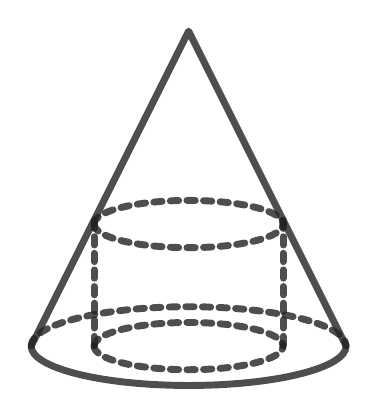
\begin{tikzpicture}[scale=1, line cap=round, line join=round]

  % Thân nón
  \draw [line width=2.5pt, color=den-2, opacity=.8] (0,0) -- (-2,-4) arc[start angle=180, end angle=360, x radius=2, y radius=0.5] -- cycle;

  % Mặt đáy nón
  \draw[dashed, line width=2.5pt, color=den-2, opacity=.8] (-2,-4) arc[start angle=180,end angle=0, x radius=2, y radius=0.5];

  % Hình trụ trong nón
  \draw[dashed, line width=2.5pt, color=den-2, opacity=.8] (-1.2,-2.4) -- (-1.2,-4);
  \draw[dashed, line width=2.5pt, color=den-2, opacity=.8] (1.2,-2.4) -- (1.2,-4);

  % Mặt đáy trụ
  % \fill[fill=yellow!50,draw=none] 
  %     (-1.2,-3) arc[start angle=180,end angle=360, x radius=1.2,y radius=0.3] -- 
  %     (1.2,-3) arc[start angle=0,end angle=180, x radius=1.2,y radius=0.3] -- cycle;

  % \draw[dashed] (-1.2,-3) arc[start angle=180, end angle=360,x radius=1.2,y radius=0.3];

  \draw[dashed, line width=2.5pt, color=den-2, opacity=.8] (-1.2,-2.45) arc[start angle=180, end angle=0, x radius=1.2, y radius=0.3];
  \draw[dashed, line width=2.5pt, color=den-2, opacity=.8] (-1.2,-2.45) arc[start angle=180, end angle=360, x radius=1.2, y radius=0.3];

  \draw[dashed, line width=2.5pt, color=den-2, opacity=.8] (-1.2,-4) arc[start angle=180, end angle=0, x radius=1.2, y radius=0.3];
  \draw[dashed, line width=2.5pt, color=den-2, opacity=.8] (-1.2,-4) arc[start angle=180, end angle=360, x radius=1.2, y radius=0.3];

  % Mặt trên trụ
  % \fill[fill=yellow!50,draw=none] 
  %     (-1.2,-2) arc[start angle=180, end angle=360, x radius=1.2,y radius=0.3] -- 
  %     (1.2,-2) arc[start angle=0, end angle=180, x radius=1.2,y radius=0.3] -- cycle;

  % \draw[dashed] (-1.2,-2) arc[start angle=180, end angle=0, x radius=1.2,y radius=0.3];

\end{tikzpicture}


\end{document}
